\documentclass[10pt]{article}
\usepackage[paperwidth=105mm,paperheight=148mm,hmargin=1cm,top=1cm,bottom=1.75cm]{geometry}
\usepackage{fontspec}
\usepackage[PunctStyle=plain]{xeCJK}
\usepackage[shortlabels,inline]{enumitem}
\usepackage{amsmath}
\usepackage{amssymb}
\usepackage{caption}
\usepackage{chemformula}
\usepackage{siunitx}
\usepackage{tikz}
\usepackage{xeCJKfntef}
\usepackage{pgfplots}
\usepackage{lastpage}
\usepackage{fancyhdr}
\usepackage{needspace}

\pretolerance=5000
\tolerance=9000
\emergencystretch=10pt

\pagestyle{fancy}
\renewcommand{\headrulewidth}{0pt}
\fancyhead{}
\cfoot{\footnotesize\thepage\ /\ \pageref{LastPage}}
\setlength{\parindent}{0pt}
\setCJKmainfont[BoldFont=Noto Serif CJK TC SemiBold]{Noto Serif CJK TC}
\linespread{1.15}

\usepackage{tabto}
\newenvironment{choice}{\begin{enumerate}[label=(\Alph*),align=left,leftmargin=*,labelsep=.3em,topsep=0ex,itemsep=0ex]}{\end{enumerate}}
%\newenvironment{choices}[1]{\par\NumTabs{#1}\begin{enumerate*}[label=(\Alph*),itemjoin=\tab]}{\end{enumerate*}}

\newcommand*{\blank}[1]{\rule[-.7\baselineskip]{0pt}{1.8\baselineskip}\fbox{\rule[-.4\baselineskip]{0pt}{1.2\baselineskip}\hspace{#1}}}
\newcommand*{\fraction}[2]{\rule[-.8\baselineskip]{0pt}{2\baselineskip}\dfrac{#1}{#2}}
\newcommand*{\sfraction}[2]{\rule[-.4\baselineskip]{0pt}{1.2\baselineskip}\tfrac{#1}{#2}}

\usepackage{titlesec}
\usepackage{zhnumber}
\titleformat{\section}{\normalfont\bfseries}{{\thesection}、}{0em}{}
\titlespacing{\section}{0pt}{2ex plus .5ex minus .2ex}{1.3ex plus .2ex}
\renewcommand{\thesection}{\zhnum{section}}

\makeatletter
\renewcommand*{\maketitle}{{%
  \bfseries
  \LARGE 練習(數學) \\
  \large 直角三角形的邊角關係 \par
}}
\makeatother

\begin{document}
\maketitle
\medskip
第 \pageref{hint} 頁設有提示,答案位於第 \pageref{answer} 頁。
\section{填充題(共 2 題)}
\begin{enumerate}[label=\Alph*.,align=left,leftmargin=*,labelsep=.3em]
  \item 如圖,在 $\triangle ABC$ 中,$\angle C = 90^\circ$,且 $\overline{AB} = 25$,$\overline{AC} = 24$。則 $\sin \angle A = \blank{5em}$,$\cos \angle A = \blank{5em}$,$\tan \angle A = \blank{5em}$。
  \begin{center}
    \begin{tikzpicture}[scale=1.5]
      \coordinate (A) at (0,0);
      \coordinate (B) at (5,0);
      \coordinate (C) at (4.608,1.344);
      \node[left] at (A) {$A$};
      \node[right] at (B) {$B$};
      \node[shift={(.2,.2)}] at (C) {$C$};
      \draw (A) -- (B) -- (C) -- (A);
    \end{tikzpicture}
  \end{center}
  \newpage
  \item 如圖,在 $\triangle ABC$ 中,$\angle B = 15^\circ$,$\angle C = 90^\circ$,且 $\overline{AC} = 1$。在 $\overline{BC}$ 上找一點 $D$,使 $\angle ADC = 30^\circ$。
  \begin{enumerate}[label=(\arabic*),left=0pt]
    \item $\overline{CD} = \blank{4em}$,$\overline{AD} = \blank{4em}$。
    \item $\angle BAD = \blank{4em}$,故 $\overline{BD} = \blank{4em}$。
    \item $\overline{AB}^2 = \blank{8em}$。(化為最簡根式)
    \item $\overline{AB} = \blank{8em}$。(化為最簡根式)
    \item $\sin 15^\circ = \fraction{\overline{AC}}{\overline{AB}} = \blank{8em}$。(化為最簡根式)
  \end{enumerate}
  \begin{center}
    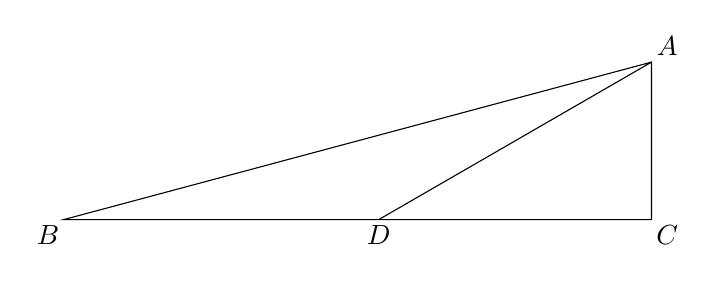
\begin{tikzpicture}
      \coordinate (A) at (0,2);
      \coordinate (B) at (-7.464,0);
      \coordinate (C) at (0,0);
      \coordinate (D) at (-3.464,0);
      \node[shift={(.2,.2)}] at (A) {$A$};
      \node[shift={(-.2,-.2)}] at (B) {$B$};
      \node[shift={(.2,-.2)}] at (C) {$C$};
      \node[shift={(0,-.2)}] at (D) {$D$};
      \draw (A) -- (B) -- (C) -- (A) -- (D);
    \end{tikzpicture}
  \end{center}
\end{enumerate}

\newpage
\label{hint}
{\bfseries\large 提示 \par}
\setcounter{section}{0}
\section{填充題}
\begin{enumerate}[label=\Alph*.,left=0pt]
  \item $\overline{AB}$ 是直角 $\triangle ABC$ 的斜邊。故 $\sin \angle A = \fraction{\overline{BC}}{\overline{AB}}$,$\cos \angle A = \fraction{\overline{AC}}{\overline{AB}}$,$\tan \angle A = \fraction{\overline{BC}}{\overline{AC}}$。
  \item
  \begin{enumerate}[label=(\arabic*),left=0pt]
    \item 利用 $\triangle ACD$ 中 $30^\circ$–$60^\circ$–$90^\circ$ 的關係。
    \item $\triangle ABD$ 是等腰三角形。
    \item 畢式定理。
    \item 需要處理雙重根號:先化為 $\sqrt{p+2\sqrt{q}}$ 的形式,接著找到 $a$ 和 $b$ 使得 $a+b=p$ 與 $ab=q$,即有 $\sqrt{p+2\sqrt{q}} = \sqrt{a} + \sqrt{b}$。
    \item 直接計算即可,需要有理化分母。
  \end{enumerate}
\end{enumerate}

\newpage
\label{answer}
{\bfseries\large 答案 \par}
\setcounter{section}{0}
\section{填充題}
\begin{enumerate}[label=\Alph*.,left=0pt]
  \item $\fraction{7}{25}$;$\fraction{24}{25}$;$\fraction{7}{24}$
  \item
  \begin{enumerate}[label=(\arabic*),left=0pt]
    \item $\sqrt{3}$;$2$
    \item $15^\circ$;$2$
    \item $8+4\sqrt{3}$
    \item $\sqrt{2}+\sqrt{6}$
    \item $\fraction{-\sqrt{2}+\sqrt{6}}{4}$
  \end{enumerate}
\end{enumerate}
\end{document}
